\documentclass{article}
\usepackage{qilin}
\hfuzz=1000pt 
\newcommand{\bff}[1]{\mathbf{#1}}
\newcommand{\image}[1]{\mathrm{im}\,#1}
\newcommand{\spann}[1]{\mathrm{span}\{#1\}}
\newcommand{\spannn}[1]{\mathrm{span}\,#1}
\newcommand{\floor}[1]{\mathrm{floor}\left(#1\right)}

% \newcommand{\dim}[1]{\mathrm{dim}\,#1}
\usepackage{blkarray}
\usepackage{pythonhighlight}
\tikzset{
  heap/.style={
    every node/.style={circle,fill=black!25,minimum size=20pt,inner sep=2pt},
    level 1/.style={sibling distance=30mm},
    level 2/.style={sibling distance=10mm}
  }
}
\newcommand{\node}[1]{
    \begin{tikzpicture}[scale=0.5, baseline=-2mm]
        \tikzstyle{vertex}=[circle,fill=black!25,outer xsep=-10pt]
        \node[vertex] (N) at (0,-0.1) {#1};
    \end{tikzpicture}
}

\title{\textbf{ESC190 Midterm Review:} \\ Data Structures and Algorithms}
\author{QiLin Xue}
\lhead{ESC190}
\rhead{QiLin Xue}

\begin{document}
    \maketitle
    \tableofcontents
    % \section{Preface}
    % In this document, I will primarily use \textit{Python} to illustrate the theory behind the different data structures. Since some portions of the midterm will be written in \textit{C}, I have done my best to write my code such that it can be easily adaptable 
    \section{Data Structures}
    \subsection{Linked List}
    A linked list uses \textit{pointers} to link from one object to another. In $C$, this is a practical way of describing lists that allow for inserting and deleting new entries, which we will call nodes. This is because we do not need to allocate this memory beforehand, which is especially handy if we do not know how large our list will be. You should be familiar with how to implement the following functions in $C$ related to linked lists:
    \begin{itemize}
        \item Creating a linked list
        \item Deleting the linked list
        \item Appending a node at a certain position
        \item Deleting a node at a certain position
        \item Finding a node which has a specific value
        \item Looking to see if there is a loop
    \end{itemize}
    The last node of a linked list should always point to the $\verb#null#$ pointer.
    \label{linked list}
    \subsection{Stacks}
    Stacks retrieve information in a \textit{last} in, \textit{first} out order.
    \inputpython{stack.py}{1}{100}

    \subsection{Queues}
    Queues retrieve information in a \textit{first} in, \textit{first} out order
    \inputpython{queue.py}{1}{100}

    \subsection{Priority Queues}
    Priority queues are similar to regular queues, except all entries are flagged with a specific weight. There are three primary operations:
    \begin{itemize}
        \item Inserting an entry and its weight into a priority queue.
        \item Find the entry with the minimum / maximum weight
        \item Retrieve the entry with the minimum / maximum weight
    \end{itemize}
    \subsection{Heaps}
    A heap is used to implement a priority queue. It takes the form of a binary tree, which can be read as a list. The only other condition for a heap is that the parent is smaller than both children. For example, $[1, 3, 9, 7, 5]$ refers to the following tree:
    \begin{center}
        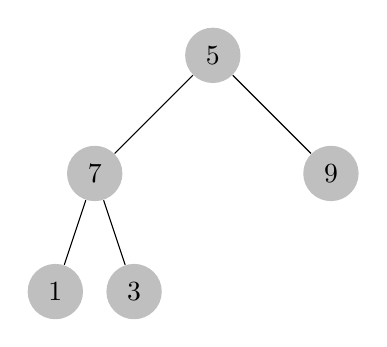
\begin{tikzpicture}[heap]
            \node {5}
            child{node{7}
              child{node{1}} child{node{3}}}
            child{node{9}}
            ;
          \end{tikzpicture}
    \end{center}
    We can denote nodes that do not have any children as \textbf{leaves}. To turn this into a heap, we start at the topmost parent, and we see if it is smaller than both its children. Since this is true, we move on to its first child \node{7}, which is bigger than both its children. As a result, we swap it with the smallest of its two children \node{1}, and we start over the same process, going back to \node{5}. Both BFS (see \ref{bfs}) and DFS (see \ref{dfs}) can be used. The following illustrates the step by step tree diagram representations of the heap.
    \begin{center}
        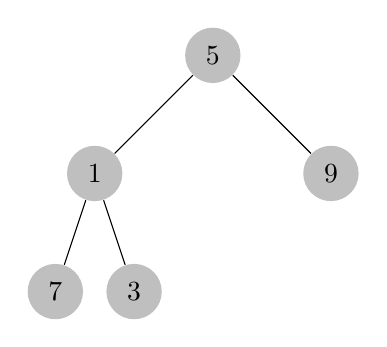
\begin{tikzpicture}[heap]
            \node {5}
            child{node{1}
              child{node{7}} child{node{3}}}
            child{node{9}}
            ;
          \end{tikzpicture}
          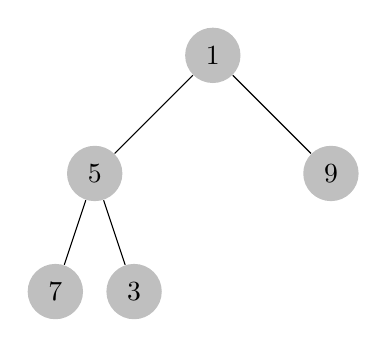
\begin{tikzpicture}[heap]
            \node {1}
            child{node{5}
              child{node{7}} child{node{3}}}
            child{node{9}}
            ;
          \end{tikzpicture}
          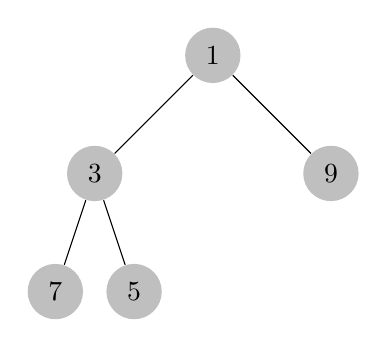
\begin{tikzpicture}[heap]
            \node {1}
            child{node{3}
              child{node{7}} child{node{5}}}
            child{node{9}}
            ;
          \end{tikzpicture}
    \end{center}
    We can use Python to verify this:
    \inputpython{heap.py}{1}{4}
    To add an element, we first place it at the next position of the tree (or the last position of the heap). We then ``percolate'' it up, comparing it with the parent until it is in the right spot. For example, suppose we wish to add \node{4}. Then the process will look like:
    \begin{center}
        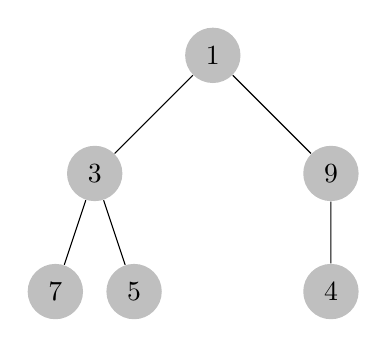
\begin{tikzpicture}[heap]
            \node {1}
            child{node{3}
              child{node{7}} child{node{5}}}
            child{node{9}child{node{4}}}
            ;
          \end{tikzpicture}
          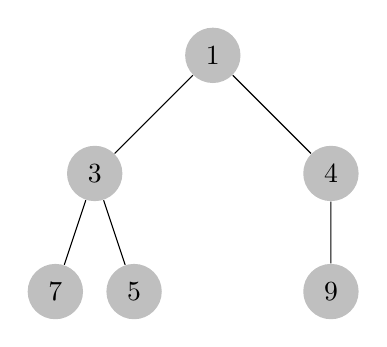
\begin{tikzpicture}[heap]
            \node {1}
            child{node{3}
              child{node{7}} child{node{5}}}
            child{node{4}child{node{9}}}
            ;
          \end{tikzpicture}
    \end{center}
    In Python, we can represent this as:
    \inputpython{heap.py}{6}{7}
    Since this is a priority queue, when we remove an element, we remove the smallest element which will always be at the very top. We can accomplish this by swapping this with the last element, and bubbling that element down. For example, suppose we wish to remove the smallest element \node{1}:
    \begin{center}
          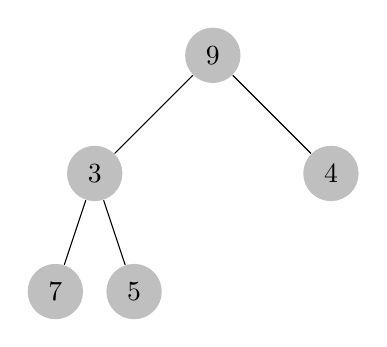
\begin{tikzpicture}[heap]
            \node {9}
            child{node{3}
              child{node{7}} child{node{5}}}
            child{node{4}}
            ;
          \end{tikzpicture}
          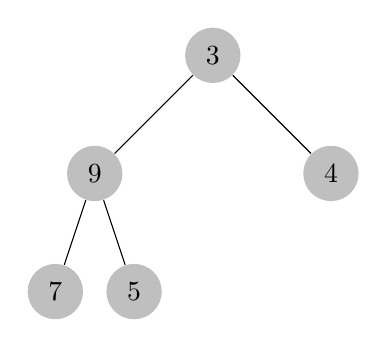
\begin{tikzpicture}[heap]
            \node {3}
            child{node{9}
              child{node{7}} child{node{5}}}
            child{node{4}}
            ;
          \end{tikzpicture}
          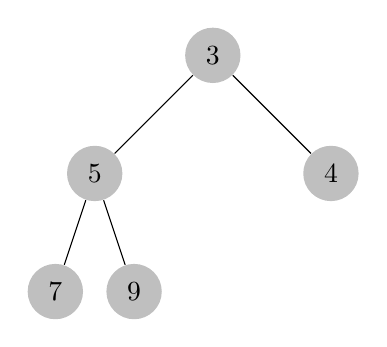
\begin{tikzpicture}[heap]
            \node {3}
            child{node{5}
              child{node{7}} child{node{9}}}
            child{node{4}}
            ;
          \end{tikzpicture}
    \end{center}
    Using Python, we have:
    \inputpython{heap.py}{9}{10}
    \subsubsection{Manual Implementation}
    Using this Python module makes working with heaps trivial and allows us to easily use a list. However, it is also possible to implement this manually with the following mathematical operations. Let the index of an element be $i$. Then:
    \begin{itemize}
        \item Index of parent: $\floor{\frac{i}{2}}$
        \item Index of left child: $2i$
        \item Index of right child: $2i+1$
    \end{itemize}
    For convention, let $i=0$ correspond to a $\verb#Null#$ element. 
    The manual implementation of heapify using Python is shown below:
    \inputpython{manual_heapify.py}{1}{100}
    \subsubsection{Runtime}
    If there are $n$ entries, then we will percolate downwards on average $n/2$ times. The time complexity of percolating downwards is $\mathcal{O}(\log n)$, so the time complexity of heaipfying a list is $\mathcal{O}(n\log n)$.

    However, it is possible to gain a better upper bound. We know that there are at least $n/2$ leaves in the heap. There are $n/4$ nodes at height $1$ (let the bottommost layer be $h=0$). There are $n/8$ nodes at height $2$, and so forth. Therefore at a height $h$, we perform:
    \begin{equation*}
        N_h \propto h \cdot \frac{n}{2^{h+1}}
    \end{equation*}
    operations such that the total number of operations is proportional to:
    \begin{equation*}
        N = \sum_{h=1}^{\log_2{n}} h \cdot \frac{n}{2^{h+1}} \propto h
    \end{equation*}
    so the total runtime is $\mathcal{O}(n)$.
    \subsubsection{Heapsort}
    We can implement a heap to sort a list with a time complexity of $\mathcal{O}(n\log n)$. We perform the following steps:
    \begin{enumerate}
        \item Create a heap from the list.
        \item Extract the minimum a total of $n$ times, and placing the elements into a list in the original order.
    \end{enumerate}
    \section{Graph Theory}
    \subsection{Background}
    \begin{itemize}
        \item We can represent a graph as $G=(V, E)$ where $V$ is the set of nodes $V=\{v_1,v_2, \dots v_n\}$ and $E$ is the set of edges $E=\{e_1, e_2, \dots, e_m\}$. 
        \item Each edge can be written as $e_k = (v_i, v_j)$.
        \item Directed graphs, or \textbf{digraphs} have edges with directions associated with them.
        \item Weighted graphs have a weight associated with each edge.
        \item Vertex $v_1$ is \textbf{adjacent} to vertex $v_2$ if an edge connects them.
        \item A \textit{path} is a sequence of vertices in which each vertex is adjacent to the next one. The length of the path is the number of edges in it.
        \item A cycle in a path is a sequence $(v_1, \dots, v_n)$ such that $(v_i, v_{i+1}) \in E$ and $(v_n, v_1) \in E$.
        \item A graph with no cycles is known as \textbf{acyclic}.
        \item A directed graph which is acyclic is known as a \textbf{DAG}.
        \item A \textbf{simple path} and a \textbf{simple cycle} has no repeated vertices.
        \item Two vertices are \textbf{connected} if there is a path between them.
        \item A subset of vertices is a connected component of a graph $G$ if each pair of vertices in the subset are connected.
        \item The \textbf{degree} of vertex $v$ is the number of edges associated with $v$.
    \end{itemize}
    \subsection{Representing Graphs}
    Suppose we take the following graph:
    \begin{center}
        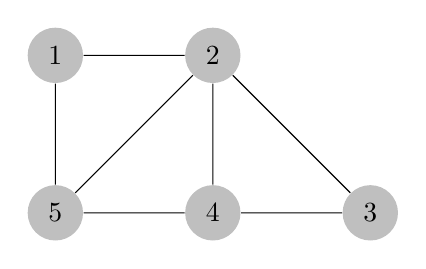
\begin{tikzpicture}[x=2cm, y=2cm]
            \tikzstyle{vertex}=[circle,fill=black!25,minimum size=20pt,inner sep=2pt]
            \node[vertex] (G_1) at (0,1)  {1};
            \node[vertex] (G_2) at (1,1)  {2};
            \node[vertex] (G_3) at (2,0)  {3};
            \node[vertex] (G_4) at (1,0)  {4};
            \node[vertex] (G_5) at (0,0)  {5};
            
            \draw (G_1) -- (G_2) -- (G_3) -- (G_4) -- (G_5) -- (G_1) -- cycle;
            \draw (G_5) -- (G_2) -- (G_4) -- cycle;
        \end{tikzpicture}
    \end{center}
    \subsubsection{Adjacency Matrix}
    For the above graph, the adjacency matrix will look like:
    \begin{equation*}
        A = \begin{blockarray}{cccccc}
            & 1 & 2 & 3 & 4 & 5 \\
            \begin{block}{c[ccccc]}
                1&0&1&0&0&1 \\ 
                2&1&0&1&1&1 \\ 
                3&0&1&0&1&0 \\ 
                4&0&1&1&0&1 \\
                5&1&1&0&1&0 \\
            \end{block}
            \end{blockarray}
    \end{equation*}
    To look up if \node{1} is connected to \node{2}, we just need to look up $\verb#A[2,1] = A[1,2]#$ (or in terms of Python notation, $\verb#A[2][1]#$ or $\verb#A[1][2]#$). Note that adjacency matrices are symmetric (e.g. $A^T = A$) for undirected graphs. It has the following complexities:
    \begin{itemize}
        \item Edge lookup: $\mathcal{O}(1)$
        \item Finding all vertices adjacent to vertex: $\mathcal{O}(|V|)$
        \item Space complexity: $\mathcal{O}(|V|^2)$
    \end{itemize}

    \subsubsection{Adjacency List}
    An adjacency list uses linked lists (see sec. \ref{linked list}) to represent the graph:
    \begin{center}
        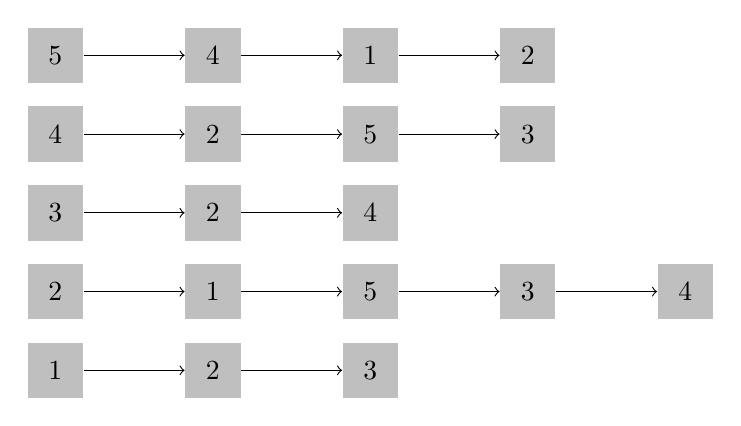
\begin{tikzpicture}[x=2cm, y=2cm]
            \tikzstyle{vertex}=[fill=black!25,minimum size=20pt,inner sep=2pt]
            \node[vertex] (A1) at (0,0)  {1};
            \node[vertex] (A2) at (1,0)  {2};
            \node[vertex] (A3) at (2,0)  {3};

            \node[vertex] (B1) at (0,0.5)  {2};
            \node[vertex] (B2) at (1,0.5)  {1};
            \node[vertex] (B3) at (2,0.5)  {5};
            \node[vertex] (B4) at (3,0.5)  {3};
            \node[vertex] (B5) at (4,0.5)  {4};
            
            \node[vertex] (C1) at (0,1)  {3};
            \node[vertex] (C2) at (1,1)  {2};
            \node[vertex] (C3) at (2,1)  {4};

            \node[vertex] (D1) at (0,1.5)  {4};
            \node[vertex] (D2) at (1,1.5)  {2};
            \node[vertex] (D3) at (2,1.5)  {5};
            \node[vertex] (D4) at (3,1.5)  {3};

            \node[vertex] (E1) at (0,2)  {5};
            \node[vertex] (E2) at (1,2)  {4};
            \node[vertex] (E3) at (2,2)  {1};
            \node[vertex] (E4) at (3,2)  {2};

            \draw[->] (A1) edge (A2) (A2) edge (A3);
            \draw[->] (B1) edge (B2) (B2) edge (B3) (B3) edge (B4) (B4) edge (B5);
            \draw[->] (C1) edge (C2) (C2) edge (C3);
            \draw[->] (D1) edge (D2) (D2) edge (D3) (D3) edge (D4);
            \draw[->] (E1) edge (E2) (E2) edge (E3) (E3) edge (E4);

        \end{tikzpicture}
    \end{center}
    This has the following complexities:
    \begin{itemize}
        \item Edge lookup: $\mathcal{O}(d)$ where $d$ is the maximum degree in the graph
        \item Finding all vertices adjacent to vertex: $\mathcal{O}(d)$
        \item Space complexity: $\mathcal{O}(|V|+|E|)$
    \end{itemize}
    \subsection{Traversal Algorithms}
    We will apply both DFS and BFS to traverse the following graph:
    \begin{center}
        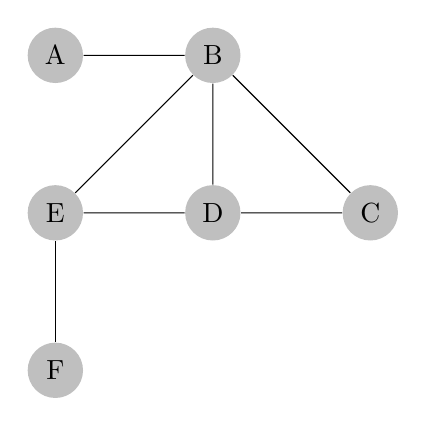
\begin{tikzpicture}[x=2cm, y=2cm]
            \tikzstyle{vertex}=[circle,fill=black!25,minimum size=20pt,inner sep=2pt]
            \node[vertex] (G_1) at (0,1)  {A};
            \node[vertex] (G_2) at (1,1)  {B};
            \node[vertex] (G_3) at (2,0)  {C};
            \node[vertex] (G_4) at (1,0)  {D};
            \node[vertex] (G_5) at (0,0)  {E};
            \node[vertex] (G_6) at (0,-1)  {F};

            \draw (G_1) -- (G_2) -- (G_3) -- (G_4) -- (G_5) -- cycle;
            \draw (G_5) -- (G_2) -- (G_4) -- cycle;
            \draw (G_5) -- (G_6) -- cycle;
        \end{tikzpicture}
    \end{center}
    We can represent this graph using Python:
    \inputpython{search.py}{1}{24}
    \subsubsection{Breadth First Search}
    To implement BFS, we use a queue. Suppose we start our search from $C$. We would explore the nodes in the following order:
    \begin{equation*}
        C \to B \to D \to A \to E \to F
    \end{equation*}
    We visit nodes in the order of the queue and every time a node is visited, the unvisited neighbours of that node is added to the back of the queue. See this Python implementation:
    \inputpython{search.py}{26}{37}
    \label{bfs}
    \subsubsection{Depth First Search}
    \label{dfs}
    In a depth first search, we make use of a stack instead. Nodes are visited in the order of the stack, and every time a node is visited, its unvisited neighbours are added to the stack. Starting from $C$, the nodes are explored in the following order:
    \begin{equation*}
        C \to D \to E \to F \to B \to A
    \end{equation*}
    which can be shown using Python:
    \inputpython{search.py}{53}{64}
    Alternatively, we can use recursion:
    \inputpython{search.py}{69}{78}
    Note that the nodes are traversed in a different order, since the implementation is slightly different. However, it is still DFS.
    \section{Shortest Path Algorithm}
    The general problem here is that we want to find the shortest path between two points through a graph. To do this, we can create a weighted graph, such as below:
    \begin{center}
        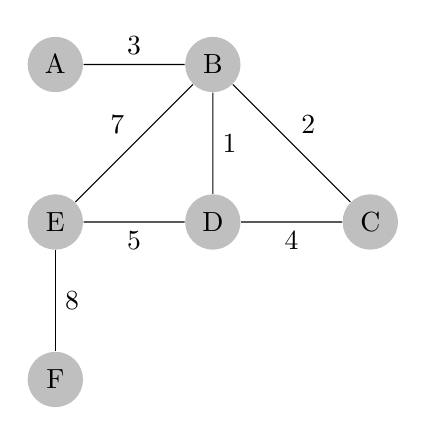
\begin{tikzpicture}[x=2cm, y=2cm]
            \tikzstyle{vertex}=[circle,fill=black!25,minimum size=20pt,inner sep=2pt]
            \node[vertex] (G_1) at (0,1)  {A};
            \node[vertex] (G_2) at (1,1)  {B};
            \node[vertex] (G_3) at (2,0)  {C};
            \node[vertex] (G_4) at (1,0)  {D};
            \node[vertex] (G_5) at (0,0)  {E};
            \node[vertex] (G_6) at (0,-1)  {F};

            \draw (G_1) -- (G_2) node[midway,above] {$3$} -- (G_3) node[midway,above right] {$2$}-- (G_4) node[midway,below] {$4$} -- (G_5) node[midway,below] {$5$} -- cycle;
            \draw (G_5) -- (G_2) node[midway,above left] {$7$} -- (G_4) node[midway,right] {$1$} -- cycle;
            \draw (G_5) -- (G_6) node[midway,right] {$8$} -- cycle;
        \end{tikzpicture}
    \end{center}
    The shortest path from \node{C} to \node{F} is $C\to B\to D \to E\to F$, but there are several paths. A weighted graph can be represented using Python as:
    \inputpython{dijkstra.py}{1}{25}
    Search functions (e.g. BFS and DFS) can be slightly modified for this slightly different data type.
    \subsection{Dijkstra's Algorithm}
    The simplest method is to apply Dijkstra's Algorithm. There are several optimizations but we will look at the simplest. The overall idea is to apply to traverse through each unexplored node. For each unexplored node, the shortest distance to each of its unexplored neighbours are set. Initially, the distance from each node to the starting node (except the starting node) is infinite:
    \begin{center}
        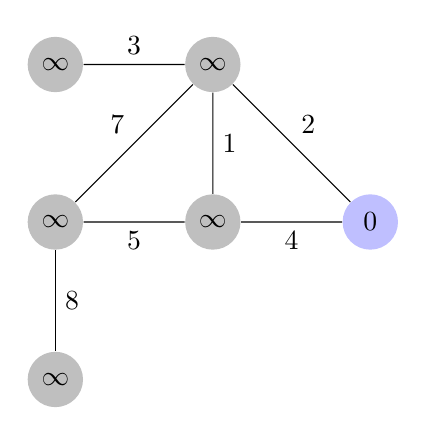
\begin{tikzpicture}[x=2cm, y=2cm]
            \tikzstyle{vertex}=[circle,fill=black!25,minimum size=20pt,inner sep=2pt]
            \tikzstyle{explored}=[circle,fill=green!25,minimum size=20pt,inner sep=2pt]
            \tikzstyle{current}=[circle,fill=blue!25,minimum size=20pt,inner sep=2pt]

            \node[vertex] (G_1) at (0,1)  {$\infty$};
            \node[vertex] (G_2) at (1,1)  {$\infty$};
            \node[current] (G_3) at (2,0)  {$0$};
            \node[vertex] (G_4) at (1,0)  {$\infty$};
            \node[vertex] (G_5) at (0,0)  {$\infty$};
            \node[vertex] (G_6) at (0,-1)  {$\infty$};

            \draw (G_1) -- (G_2) node[midway,above] {$3$} -- (G_3) node[midway,above right] {$2$}-- (G_4) node[midway,below] {$4$} -- (G_5) node[midway,below] {$5$} -- cycle;
            \draw (G_5) -- (G_2) node[midway,above left] {$7$} -- (G_4) node[midway,right] {$1$} -- cycle;
            \draw (G_5) -- (G_6) node[midway,right] {$8$} -- cycle;
        \end{tikzpicture}
    \end{center}
    Here, a blue node represents the node we are currently exploring and nodes that we have already explored will be drawn as green.
    \begin{center}
    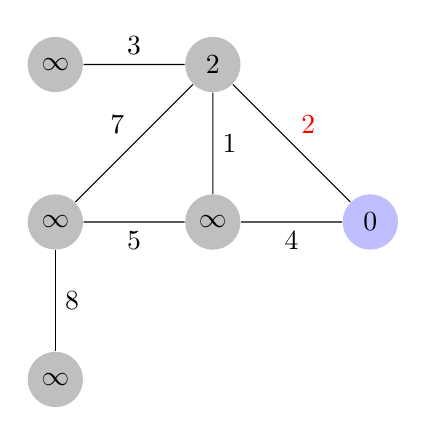
\begin{tikzpicture}[x=2cm, y=2cm]
        \tikzstyle{vertex}=[circle,fill=black!25,minimum size=20pt,inner sep=2pt]
        \tikzstyle{explored}=[circle,fill=green!25,minimum size=20pt,inner sep=2pt]
        \tikzstyle{current}=[circle,fill=blue!25,minimum size=20pt,inner sep=2pt]

        \node[vertex] (G_1) at (0,1)  {$\infty$};
        \node[vertex] (G_2) at (1,1)  {$2$};
        \node[current] (G_3) at (2,0)  {$0$};
        \node[vertex] (G_4) at (1,0)  {$\infty$};
        \node[vertex] (G_5) at (0,0)  {$\infty$};
        \node[vertex] (G_6) at (0,-1)  {$\infty$};

        \draw (G_1) -- (G_2) node[midway,above] {$3$} -- (G_3) node[midway,above right,red] {$2$}-- (G_4) node[midway,below] {$4$} -- (G_5) node[midway,below] {$5$} -- cycle;
        \draw (G_5) -- (G_2) node[midway,above left] {$7$} -- (G_4) node[midway,right] {$1$} -- cycle;
        \draw (G_5) -- (G_6) node[midway,right] {$8$} -- cycle;
    \end{tikzpicture}\hspace{2mm}
    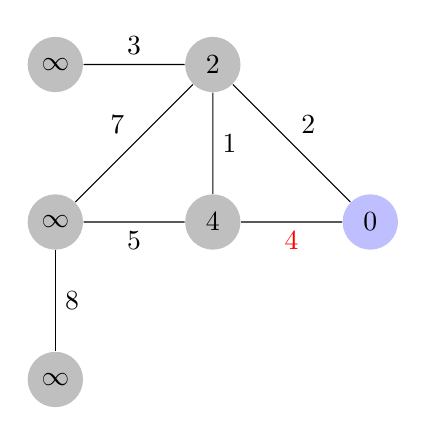
\begin{tikzpicture}[x=2cm, y=2cm]
        \tikzstyle{vertex}=[circle,fill=black!25,minimum size=20pt,inner sep=2pt]
        \tikzstyle{explored}=[circle,fill=green!25,minimum size=20pt,inner sep=2pt]
        \tikzstyle{current}=[circle,fill=blue!25,minimum size=20pt,inner sep=2pt]

        \node[vertex] (G_1) at (0,1)  {$\infty$};
        \node[vertex] (G_2) at (1,1)  {$2$};
        \node[current] (G_3) at (2,0)  {$0$};
        \node[vertex] (G_4) at (1,0)  {$4$};
        \node[vertex] (G_5) at (0,0)  {$\infty$};
        \node[vertex] (G_6) at (0,-1)  {$\infty$};

        \draw (G_1) -- (G_2) node[midway,above] {$3$} -- (G_3) node[midway,above right] {$2$}-- (G_4) node[midway,below,red] {$4$} -- (G_5) node[midway,below] {$5$} -- cycle;
        \draw (G_5) -- (G_2) node[midway,above left] {$7$} -- (G_4) node[midway,right] {$1$} -- cycle;
        \draw (G_5) -- (G_6) node[midway,right] {$8$} -- cycle;
    \end{tikzpicture}
    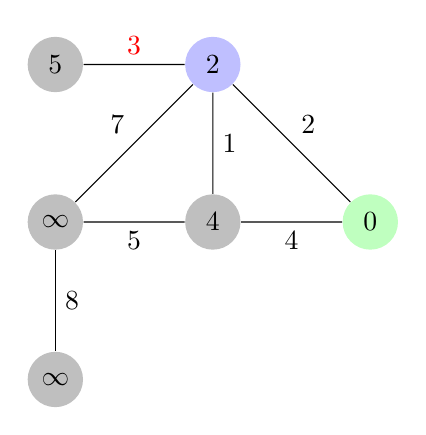
\begin{tikzpicture}[x=2cm, y=2cm]
        \tikzstyle{vertex}=[circle,fill=black!25,minimum size=20pt,inner sep=2pt]
        \tikzstyle{explored}=[circle,fill=green!25,minimum size=20pt,inner sep=2pt]
        \tikzstyle{current}=[circle,fill=blue!25,minimum size=20pt,inner sep=2pt]

        \node[vertex] (G_1) at (0,1)  {$5$};
        \node[current] (G_2) at (1,1)  {$2$};
        \node[explored] (G_3) at (2,0)  {$0$};
        \node[vertex] (G_4) at (1,0)  {$4$};
        \node[vertex] (G_5) at (0,0)  {$\infty$};
        \node[vertex] (G_6) at (0,-1)  {$\infty$};

        \draw (G_1) -- (G_2) node[midway,above,red] {$3$} -- (G_3) node[midway,above right] {$2$}-- (G_4) node[midway,below] {$4$} -- (G_5) node[midway,below] {$5$} -- cycle;
        \draw (G_5) -- (G_2) node[midway,above left] {$7$} -- (G_4) node[midway,right] {$1$} -- cycle;
        \draw (G_5) -- (G_6) node[midway,right] {$8$} -- cycle;
    \end{tikzpicture}
    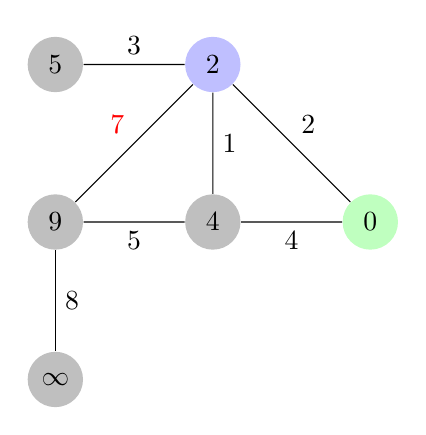
\begin{tikzpicture}[x=2cm, y=2cm]
        \tikzstyle{vertex}=[circle,fill=black!25,minimum size=20pt,inner sep=2pt]
        \tikzstyle{explored}=[circle,fill=green!25,minimum size=20pt,inner sep=2pt]
        \tikzstyle{current}=[circle,fill=blue!25,minimum size=20pt,inner sep=2pt]

        \node[vertex] (G_1) at (0,1)  {$5$};
        \node[current] (G_2) at (1,1)  {$2$};
        \node[explored] (G_3) at (2,0)  {$0$};
        \node[vertex] (G_4) at (1,0)  {$4$};
        \node[vertex] (G_5) at (0,0)  {$9$};
        \node[vertex] (G_6) at (0,-1)  {$\infty$};

        \draw (G_1) -- (G_2) node[midway,above] {$3$} -- (G_3) node[midway,above right] {$2$}-- (G_4) node[midway,below] {$4$} -- (G_5) node[midway,below] {$5$} -- cycle;
        \draw (G_5) -- (G_2) node[midway,above left,red] {$7$} -- (G_4) node[midway,right] {$1$} -- cycle;
        \draw (G_5) -- (G_6) node[midway,right] {$8$} -- cycle;
    \end{tikzpicture}
    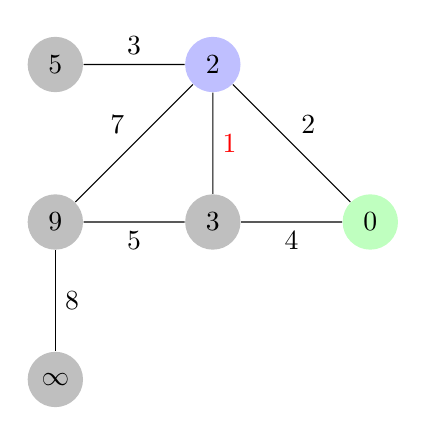
\begin{tikzpicture}[x=2cm, y=2cm]
        \tikzstyle{vertex}=[circle,fill=black!25,minimum size=20pt,inner sep=2pt]
        \tikzstyle{explored}=[circle,fill=green!25,minimum size=20pt,inner sep=2pt]
        \tikzstyle{current}=[circle,fill=blue!25,minimum size=20pt,inner sep=2pt]

        \node[vertex] (G_1) at (0,1)  {$5$};
        \node[current] (G_2) at (1,1)  {$2$};
        \node[explored] (G_3) at (2,0)  {$0$};
        \node[vertex] (G_4) at (1,0)  {$3$};
        \node[vertex] (G_5) at (0,0)  {$9$};
        \node[vertex] (G_6) at (0,-1)  {$\infty$};

        \draw (G_1) -- (G_2) node[midway,above] {$3$} -- (G_3) node[midway,above right] {$2$}-- (G_4) node[midway,below] {$4$} -- (G_5) node[midway,below] {$5$} -- cycle;
        \draw (G_5) -- (G_2) node[midway,above left] {$7$} -- (G_4) node[midway,right,red] {$1$} -- cycle;
        \draw (G_5) -- (G_6) node[midway,right] {$8$} -- cycle;
    \end{tikzpicture}
    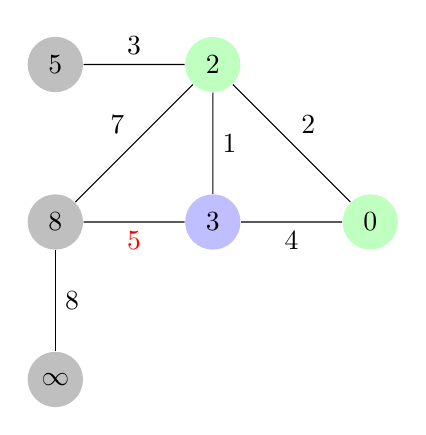
\begin{tikzpicture}[x=2cm, y=2cm]
        \tikzstyle{vertex}=[circle,fill=black!25,minimum size=20pt,inner sep=2pt]
        \tikzstyle{explored}=[circle,fill=green!25,minimum size=20pt,inner sep=2pt]
        \tikzstyle{current}=[circle,fill=blue!25,minimum size=20pt,inner sep=2pt]

        \node[vertex] (G_1) at (0,1)  {$5$};
        \node[explored] (G_2) at (1,1)  {$2$};
        \node[explored] (G_3) at (2,0)  {$0$};
        \node[current] (G_4) at (1,0)  {$3$};
        \node[vertex] (G_5) at (0,0)  {$8$};
        \node[vertex] (G_6) at (0,-1)  {$\infty$};

        \draw (G_1) -- (G_2) node[midway,above] {$3$} -- (G_3) node[midway,above right] {$2$}-- (G_4) node[midway,below] {$4$} -- (G_5) node[midway,below,red] {$5$} -- cycle;
        \draw (G_5) -- (G_2) node[midway,above left] {$7$} -- (G_4) node[midway,right] {$1$} -- cycle;
        \draw (G_5) -- (G_6) node[midway,right] {$8$} -- cycle;
    \end{tikzpicture}
    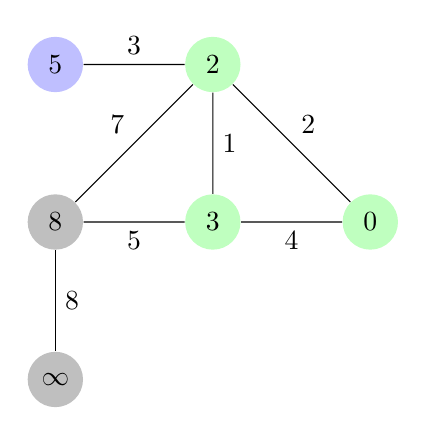
\begin{tikzpicture}[x=2cm, y=2cm]
        \tikzstyle{vertex}=[circle,fill=black!25,minimum size=20pt,inner sep=2pt]
        \tikzstyle{explored}=[circle,fill=green!25,minimum size=20pt,inner sep=2pt]
        \tikzstyle{current}=[circle,fill=blue!25,minimum size=20pt,inner sep=2pt]

        \node[current] (G_1) at (0,1)  {$5$};
        \node[explored] (G_2) at (1,1)  {$2$};
        \node[explored] (G_3) at (2,0)  {$0$};
        \node[explored] (G_4) at (1,0)  {$3$};
        \node[vertex] (G_5) at (0,0)  {$8$};
        \node[vertex] (G_6) at (0,-1)  {$\infty$};

        \draw (G_1) -- (G_2) node[midway,above] {$3$} -- (G_3) node[midway,above right] {$2$}-- (G_4) node[midway,below] {$4$} -- (G_5) node[midway,below] {$5$} -- cycle;
        \draw (G_5) -- (G_2) node[midway,above left] {$7$} -- (G_4) node[midway,right] {$1$} -- cycle;
        \draw (G_5) -- (G_6) node[midway,right] {$8$} -- cycle;
    \end{tikzpicture}
    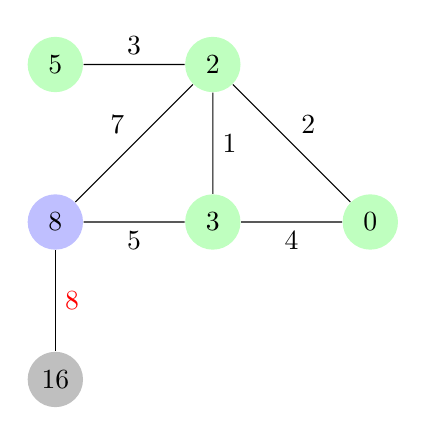
\begin{tikzpicture}[x=2cm, y=2cm]
        \tikzstyle{vertex}=[circle,fill=black!25,minimum size=20pt,inner sep=2pt]
        \tikzstyle{explored}=[circle,fill=green!25,minimum size=20pt,inner sep=2pt]
        \tikzstyle{current}=[circle,fill=blue!25,minimum size=20pt,inner sep=2pt]

        \node[explored] (G_1) at (0,1)  {$5$};
        \node[explored] (G_2) at (1,1)  {$2$};
        \node[explored] (G_3) at (2,0)  {$0$};
        \node[explored] (G_4) at (1,0)  {$3$};
        \node[current] (G_5) at (0,0)  {$8$};
        \node[vertex] (G_6) at (0,-1)  {$16$};

        \draw (G_1) -- (G_2) node[midway,above] {$3$} -- (G_3) node[midway,above right] {$2$}-- (G_4) node[midway,below] {$4$} -- (G_5) node[midway,below] {$5$} -- cycle;
        \draw (G_5) -- (G_2) node[midway,above left] {$7$} -- (G_4) node[midway,right] {$1$} -- cycle;
        \draw (G_5) -- (G_6) node[midway,right,red] {$8$} -- cycle;
    \end{tikzpicture}
    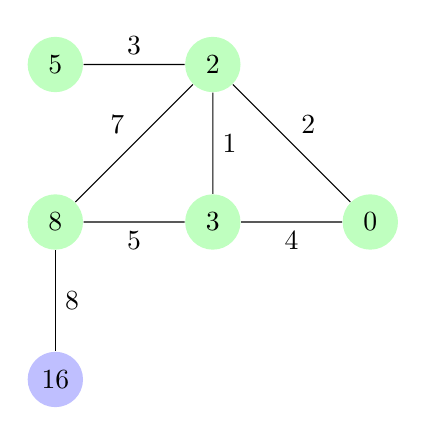
\begin{tikzpicture}[x=2cm, y=2cm]
        \tikzstyle{vertex}=[circle,fill=black!25,minimum size=20pt,inner sep=2pt]
        \tikzstyle{explored}=[circle,fill=green!25,minimum size=20pt,inner sep=2pt]
        \tikzstyle{current}=[circle,fill=blue!25,minimum size=20pt,inner sep=2pt]

        \node[explored] (G_1) at (0,1)  {$5$};
        \node[explored] (G_2) at (1,1)  {$2$};
        \node[explored] (G_3) at (2,0)  {$0$};
        \node[explored] (G_4) at (1,0)  {$3$};
        \node[explored] (G_5) at (0,0)  {$8$};
        \node[current] (G_6) at (0,-1)  {$16$};

        \draw (G_1) -- (G_2) node[midway,above] {$3$} -- (G_3) node[midway,above right] {$2$}-- (G_4) node[midway,below] {$4$} -- (G_5) node[midway,below] {$5$} -- cycle;
        \draw (G_5) -- (G_2) node[midway,above left] {$7$} -- (G_4) node[midway,right] {$1$} -- cycle;
        \draw (G_5) -- (G_6) node[midway,right] {$8$} -- cycle;
    \end{tikzpicture}
    \end{center}
    We can show this below via Python:
    \inputpython{dijkstra.py}{27}{67}
    To obtain the path, we can implement a dictionary \pyth{prev} and whenever the path to a certain node improves, we call: \pyth{prev[con["node"].name] = cur.name}.

    To add one vertex to $S$, we must search through all possible vertices so the runtime complexity is $\mathcal{O}(|V|^2)$.
    \subsection{Using Priority Queue}
    It is possible to improve the runtime to $\mathcal{O}(|E|\log |V|)$ using a priority queue:
    \inputpython{dijkstra.py}{71}{115}
    This algorithm is essentially the same, but instead of traversing explored nodes via BFS, we traverse it by sorting the nodes by their distance from the origin. The upper bound on the number of times a node is pushed is $2|E|$ and popping/pushing into \pyth{pq} has a time complexity of $\mathcal{O}(\log|V|)$. The time complexity of this algorithm is thus $\mathcal{O}(|E|\log|V|)$.
    \subsection{Greedy Best First Search}
    The general theme of search algorithms is to select a way to traverse explored nodes. In the simple method, it was via BFS. In the priority queue method, it was prioritizing nodes with a smaller distance. In the greedy best first search, it is by using a heuristic function $h(v)$ that gives a rough estimate of the distance between a node and the destination.

    For example, take the below graph and suppose we wish to move from \node{C} to \node{A}. Unlike the previous examples, the length of each path corresponds to their weights, so we can imagine these as physical points in space. We can let our heuristic function be the \textit{Manhattan distance} $\Delta x + \Delta y$:
    \begin{center}
        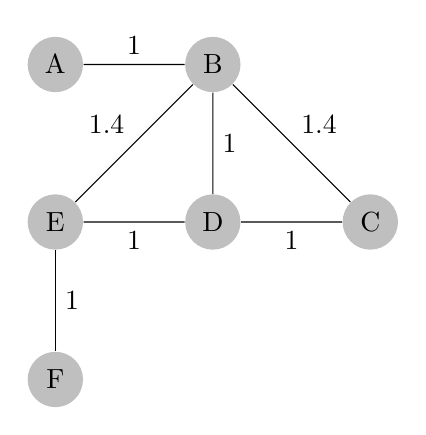
\begin{tikzpicture}[x=2cm, y=2cm]
            \tikzstyle{vertex}=[circle,fill=black!25,minimum size=20pt,inner sep=2pt]
            \node[vertex] (G_1) at (0,1)  {A};
            \node[vertex] (G_2) at (1,1)  {B};
            \node[vertex] (G_3) at (2,0)  {C};
            \node[vertex] (G_4) at (1,0)  {D};
            \node[vertex] (G_5) at (0,0)  {E};
            \node[vertex] (G_6) at (0,-1)  {F};

            \draw (G_1) -- (G_2) node[midway,above] {$1$} -- (G_3) node[midway,above right] {$1.4$}-- (G_4) node[midway,below] {$1$} -- (G_5) node[midway,below] {$1$} -- cycle;
            \draw (G_5) -- (G_2) node[midway,above left] {$1.4$} -- (G_4) node[midway,right] {$1$} -- cycle;
            \draw (G_5) -- (G_6) node[midway,right] {$1$} -- cycle;
        \end{tikzpicture}
    \end{center}
    We will start from \node{C} and look at the neighbours. The neighbour that minimizes the Manhattan distance is \node{B}, which directly leads to \node{A}. As you can expect, this is \textit{really bad}. It doesn't even bother checking if going to \node{D} is faster, but if we have a good heuristic, this isn't necessary. We can implement it in Python below:
    \inputpython{greedy.py}{1}{64}
    \subsection{A*}
    The A* algorithm is more robust, and combines the advantages of using a heuristic function with a priority queue. It is extremely similar to the optimized version of dijkstra's, except the priority queue is sorted by the heuristic function. We can also implement it in Python:
    \inputpython{A.py}{1}{61}
\end{document}
